\documentclass[12pt]{report}\usepackage[]{graphicx}\usepackage[dvipsnames]{xcolor}
% maxwidth is the original width if it is less than linewidth
% otherwise use linewidth (to make sure the graphics do not exceed the margin)
\makeatletter
\def\maxwidth{ %
  \ifdim\Gin@nat@width>\linewidth
    \linewidth
  \else
    \Gin@nat@width
  \fi
}
\makeatother

\definecolor{fgcolor}{rgb}{0.345, 0.345, 0.345}
\newcommand{\hlnum}[1]{\textcolor[rgb]{0.686,0.059,0.569}{#1}}%
\newcommand{\hlstr}[1]{\textcolor[rgb]{0.192,0.494,0.8}{#1}}%
\newcommand{\hlcom}[1]{\textcolor[rgb]{0.678,0.584,0.686}{\textit{#1}}}%
\newcommand{\hlopt}[1]{\textcolor[rgb]{0,0,0}{#1}}%
\newcommand{\hlstd}[1]{\textcolor[rgb]{0.345,0.345,0.345}{#1}}%
\newcommand{\hlkwa}[1]{\textcolor[rgb]{0.161,0.373,0.58}{\textbf{#1}}}%
\newcommand{\hlkwb}[1]{\textcolor[rgb]{0.69,0.353,0.396}{#1}}%
\newcommand{\hlkwc}[1]{\textcolor[rgb]{0.333,0.667,0.333}{#1}}%
\newcommand{\hlkwd}[1]{\textcolor[rgb]{0.737,0.353,0.396}{\textbf{#1}}}%
\let\hlipl\hlkwb

\usepackage{framed}
\makeatletter
\newenvironment{kframe}{%
 \def\at@end@of@kframe{}%
 \ifinner\ifhmode%
  \def\at@end@of@kframe{\end{minipage}}%
  \begin{minipage}{\columnwidth}%
 \fi\fi%
 \def\FrameCommand##1{\hskip\@totalleftmargin \hskip-\fboxsep
 \colorbox{shadecolor}{##1}\hskip-\fboxsep
     % There is no \\@totalrightmargin, so:
     \hskip-\linewidth \hskip-\@totalleftmargin \hskip\columnwidth}%
 \MakeFramed {\advance\hsize-\width
   \@totalleftmargin\z@ \linewidth\hsize
   \@setminipage}}%
 {\par\unskip\endMakeFramed%
 \at@end@of@kframe}
\makeatother

\definecolor{shadecolor}{rgb}{.97, .97, .97}
\definecolor{messagecolor}{rgb}{0, 0, 0}
\definecolor{warningcolor}{rgb}{1, 0, 1}
\definecolor{errorcolor}{rgb}{1, 0, 0}
\newenvironment{knitrout}{}{} % an empty environment to be redefined in TeX

\usepackage{alltt}

\usepackage[utf8]{inputenc}
\usepackage[spanish]{babel}
\usepackage[margin=2.54cm]{geometry}
\usepackage[dvipsnames]{xcolor}
\usepackage{array, amssymb, amsthm, enumitem, fancyhdr, float, graphicx, hyperref, hologo, mathtools, tikz, tikz-cd}
\usepackage[spanish, noabbrev]{cleveref}

\pagestyle{fancy}
\lhead{\footnotesize \leftmark}
\rhead{\footnotesize \rightmark}

\title{
	\huge
	\noindent\textbf{Fundamentos de la Ciencia de Datos}\\
	
	{\Large \textit{Práctica 1}}
	\vspace{1cm}
	
	\huge
	Grado en Ingeniería Informática\\
	Universidad de Alcalá\\
	
	\vspace{1cm}
	
	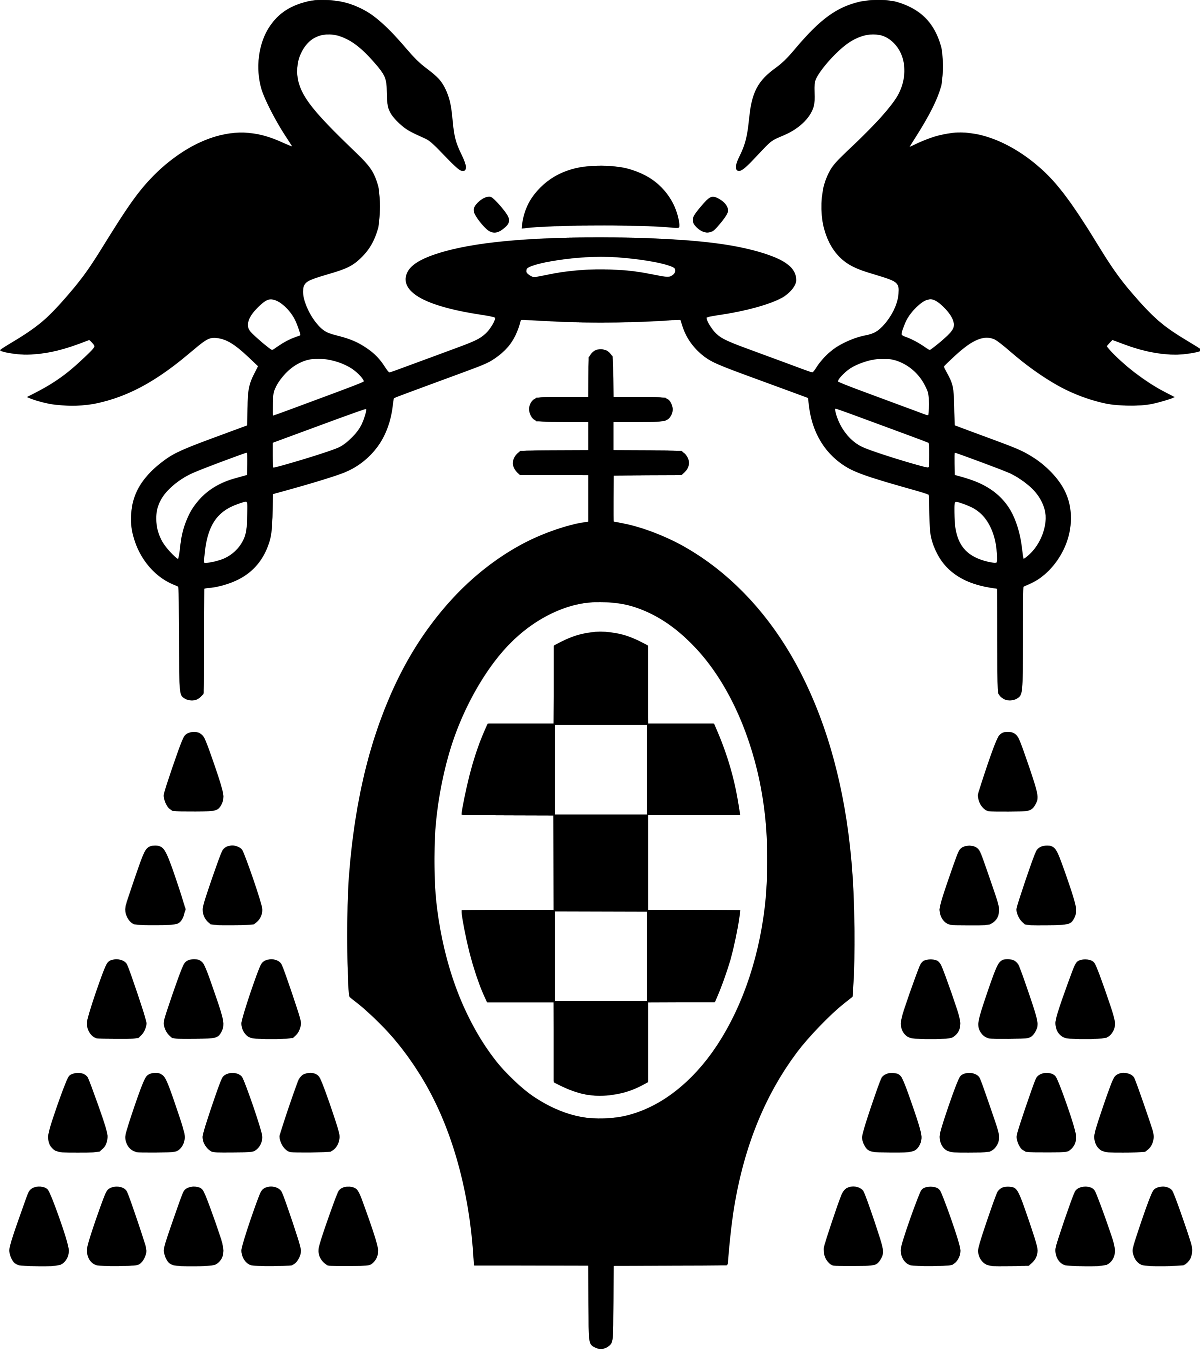
\includegraphics[scale=0.075]{img/logo}
}

\author{
	Pablo García García\\
	Abel López Martínez\\
	Álvaro Jesús Martínez Parra\\
	Raúl Moratilla Núñez
}

\date{
	\large{14 de noviembre de 2023}
}

\hypersetup{
	pdftitle={Práctica 1}, 
	pdfauthor={Pablo García García, Abel López Martínez, Álvaro Jesús Martínez Parra, Raúl Moratilla Núñez}, 
	pdfsubject={Fundamentos de la Ciencia de Datos}, 
	pdfcenterwindow, 
	pdfnewwindow=true, 
	pdfkeywords={Entrega de la PL1 de laboratorio correspondiente al Curso 2023-2024}, 
	bookmarksopen=true 
}
\IfFileExists{upquote.sty}{\usepackage{upquote}}{}
\begin{document}
	
\begin{knitrout}
\definecolor{shadecolor}{rgb}{0.969, 0.969, 0.969}\color{fgcolor}\begin{kframe}
\begin{alltt}
\hlstd{fichero} \hlkwb{=} \hlkwd{read.csv}\hlstd{(}\hlstr{"distancia_universitarios.csv"}\hlstd{)}
\hlstd{fichero}
\end{alltt}
\begin{verbatim}
##    Distancia
## 1       16.5
## 2       34.8
## 3       20.7
## 4        6.2
## 5        4.4
## 6        3.4
## 7       24.0
## 8       24.0
## 9       32.0
## 10      30.0
## 11      33.0
## 12      27.0
## 13      15.0
## 14       9.4
## 15       2.1
## 16      34.0
## 17      24.0
## 18      12.0
## 19       4.4
## 20      28.0
## 21      31.4
## 22      21.6
## 23       3.1
## 24       4.5
## 25       5.1
## 26       4.0
## 27       3.2
## 28      25.0
## 29       4.5
## 30      20.0
## 31      34.0
## 32      12.0
## 33      12.0
## 34      12.0
## 35      12.0
## 36       5.0
## 37      19.0
## 38      30.0
## 39       5.5
## 40      38.0
## 41      25.0
## 42       3.7
## 43       9.0
## 44      30.0
## 45      13.0
## 46      30.0
## 47      30.0
## 48      26.0
## 49      30.0
## 50      30.0
## 51       1.0
## 52      26.0
## 53      22.0
## 54      10.0
## 55       9.7
## 56      11.0
## 57      24.1
## 58      33.0
## 59      17.2
## 60      27.0
## 61      24.0
## 62      27.0
## 63      21.0
## 64      28.0
## 65      30.0
## 66       4.0
## 67      46.0
## 68      29.0
## 69       3.7
## 70       2.7
## 71       8.1
## 72      19.0
## 73      16.0
\end{verbatim}
\begin{alltt}
\hlstd{len} \hlkwb{=} \hlkwa{function}\hlstd{(}\hlkwc{list}\hlstd{)\{}
        \hlstd{count} \hlkwb{=} \hlnum{0}
        \hlkwa{for} \hlstd{(element} \hlkwa{in} \hlstd{list)\{}
                \hlstd{count} \hlkwb{=} \hlstd{count} \hlopt{+} \hlnum{1}
        \hlstd{\}}
        \hlstd{count}
\hlstd{\}}

\hlstd{distancias} \hlkwb{=} \hlstd{fichero}\hlopt{$}\hlstd{Distancia}

\hlstd{longitud} \hlkwb{=} \hlkwd{len}\hlstd{(distancias)}
\hlstd{longitud}
\end{alltt}
\begin{verbatim}
## [1] 73
\end{verbatim}
\begin{alltt}
\hlstd{bubble} \hlkwb{=} \hlkwa{function}\hlstd{(}\hlkwc{list}\hlstd{,} \hlkwc{asc} \hlstd{=} \hlnum{TRUE}\hlstd{)\{}
        \hlstd{n} \hlkwb{=} \hlkwd{len}\hlstd{(list)}
        \hlkwa{if}\hlstd{(asc)\{}
                \hlkwa{for} \hlstd{(i} \hlkwa{in} \hlnum{2}\hlopt{:}\hlstd{n)\{}
                        \hlkwa{for} \hlstd{(j} \hlkwa{in} \hlnum{1}\hlopt{:}\hlstd{(n}\hlopt{-}\hlnum{1}\hlstd{))\{}
                                \hlkwa{if} \hlstd{(list[j]} \hlopt{>} \hlstd{list[j}\hlopt{+}\hlnum{1}\hlstd{])\{}
                                        \hlstd{temp} \hlkwb{=} \hlstd{list[j]}
                                        \hlstd{list[j]} \hlkwb{=} \hlstd{list[j}\hlopt{+}\hlnum{1}\hlstd{]}
                                        \hlstd{list[j}\hlopt{+}\hlnum{1}\hlstd{]} \hlkwb{=} \hlstd{temp}
                                \hlstd{\}}
                        \hlstd{\}}
                \hlstd{\}}
        \hlstd{\}}
        \hlkwa{else} \hlstd{\{}
                \hlkwa{for} \hlstd{(i} \hlkwa{in} \hlnum{2}\hlopt{:}\hlstd{n)\{}
                        \hlkwa{for} \hlstd{(j} \hlkwa{in} \hlnum{1}\hlopt{:}\hlstd{(n}\hlopt{-}\hlnum{1}\hlstd{))\{}
                                \hlkwa{if} \hlstd{(list[j]} \hlopt{<} \hlstd{list[j}\hlopt{+}\hlnum{1}\hlstd{])\{}
                                        \hlstd{temp} \hlkwb{=} \hlstd{list[j]}
                                        \hlstd{list[j]} \hlkwb{=} \hlstd{list[j}\hlopt{+}\hlnum{1}\hlstd{]}
                                        \hlstd{list[j}\hlopt{+}\hlnum{1}\hlstd{]} \hlkwb{=} \hlstd{temp}
                                \hlstd{\}}
                        \hlstd{\}}
                \hlstd{\}}
        \hlstd{\}}
        \hlstd{list}
\hlstd{\}}
\hlstd{distanciasordenadas} \hlkwb{=} \hlkwd{bubble}\hlstd{(distancias,} \hlnum{FALSE}\hlstd{)}
\hlstd{distanciasordenadas}
\end{alltt}
\begin{verbatim}
##  [1] 46.0 38.0 34.8 34.0 34.0 33.0 33.0 32.0 31.4 30.0 30.0 30.0 30.0 30.0 30.0
## [16] 30.0 30.0 29.0 28.0 28.0 27.0 27.0 27.0 26.0 26.0 25.0 25.0 24.1 24.0 24.0
## [31] 24.0 24.0 22.0 21.6 21.0 20.7 20.0 19.0 19.0 17.2 16.5 16.0 15.0 13.0 12.0
## [46] 12.0 12.0 12.0 12.0 11.0 10.0  9.7  9.4  9.0  8.1  6.2  5.5  5.1  5.0  4.5
## [61]  4.5  4.4  4.4  4.0  4.0  3.7  3.7  3.4  3.2  3.1  2.7  2.1  1.0
\end{verbatim}
\begin{alltt}
\hlstd{rank} \hlkwb{=} \hlkwa{function}\hlstd{(}\hlkwc{list}\hlstd{)\{}
        \hlstd{ordered_list} \hlkwb{=} \hlkwd{bubble}\hlstd{(list)}
        \hlstd{ordered_list[}\hlkwd{len}\hlstd{(ordered_list)]} \hlopt{-} \hlstd{ordered_list[}\hlnum{1}\hlstd{]}
\hlstd{\}}

\hlstd{rango} \hlkwb{=} \hlkwd{rank}\hlstd{(distanciasordenadas)}
\hlstd{rango}
\end{alltt}
\begin{verbatim}
## [1] 45
\end{verbatim}
\begin{alltt}
\hlstd{absolute_freq} \hlkwb{=} \hlkwa{function}\hlstd{(}\hlkwc{list}\hlstd{)\{}
        \hlstd{ordered_list} \hlkwb{=} \hlkwd{bubble}\hlstd{(list)}
        \hlstd{n} \hlkwb{=} \hlkwd{len}\hlstd{(ordered_list)}
        \hlstd{elements} \hlkwb{=} \hlkwd{vector}\hlstd{()}
        \hlstd{frequencies} \hlkwb{=} \hlkwd{vector}\hlstd{()}
        \hlstd{i} \hlkwb{=} \hlnum{1}
        \hlkwa{while} \hlstd{(i} \hlopt{<=} \hlstd{n)\{}
                \hlstd{actual_element} \hlkwb{=} \hlstd{ordered_list[i]}
                \hlstd{elements} \hlkwb{=} \hlkwd{append}\hlstd{(elements, actual_element)}
                \hlstd{actual_freq} \hlkwb{=} \hlnum{0}
                \hlstd{j} \hlkwb{=} \hlstd{i}
                \hlkwa{while}\hlstd{(j} \hlopt{<=} \hlstd{n} \hlopt{&} \hlstd{actual_element} \hlopt{==} \hlstd{ordered_list[j])\{}
                        \hlstd{actual_freq} \hlkwb{=} \hlstd{actual_freq} \hlopt{+} \hlnum{1}
                        \hlstd{j} \hlkwb{=} \hlstd{j}\hlopt{+}\hlnum{1}
                \hlstd{\}}
                \hlstd{frequencies} \hlkwb{=} \hlkwd{append}\hlstd{(frequencies, actual_freq)}
                \hlstd{i} \hlkwb{=} \hlstd{j}
        \hlstd{\}}
        \hlkwd{rbind}\hlstd{(elements, frequencies)}
\hlstd{\}}
\hlstd{frecuencia_abs} \hlkwb{=} \hlkwd{absolute_freq}\hlstd{(distancias)}
\hlstd{frecuencia_abs}
\end{alltt}
\begin{verbatim}
##             [,1] [,2] [,3] [,4] [,5] [,6] [,7] [,8] [,9] [,10] [,11] [,12]
## elements       1  2.1  2.7  3.1  3.2  3.4  3.7    4  4.4   4.5     5   5.1
## frequencies    1  1.0  1.0  1.0  1.0  1.0  2.0    2  2.0   2.0     1   1.0
##             [,13] [,14] [,15] [,16] [,17] [,18] [,19] [,20] [,21] [,22] [,23]
## elements      5.5   6.2   8.1     9   9.4   9.7    10    11    12    13    15
## frequencies   1.0   1.0   1.0     1   1.0   1.0     1     1     5     1     1
##             [,24] [,25] [,26] [,27] [,28] [,29] [,30] [,31] [,32] [,33] [,34]
## elements       16  16.5  17.2    19    20  20.7    21  21.6    22    24  24.1
## frequencies     1   1.0   1.0     2     1   1.0     1   1.0     1     4   1.0
##             [,35] [,36] [,37] [,38] [,39] [,40] [,41] [,42] [,43] [,44] [,45]
## elements       25    26    27    28    29    30  31.4    32    33    34  34.8
## frequencies     2     2     3     2     1     8   1.0     1     2     2   1.0
##             [,46] [,47]
## elements       38    46
## frequencies     1     1
\end{verbatim}
\begin{alltt}
\hlstd{relative_freq} \hlkwb{=} \hlkwa{function}\hlstd{(}\hlkwc{list}\hlstd{)\{}
        \hlstd{f_abs} \hlkwb{=} \hlkwd{absolute_freq}\hlstd{(list)}
        \hlstd{elements} \hlkwb{=} \hlstd{f_abs[}\hlnum{1}\hlstd{,]}
        \hlstd{abs_fvalues} \hlkwb{=} \hlstd{f_abs[}\hlnum{2}\hlstd{,]}
        \hlkwd{rbind}\hlstd{(elements,abs_fvalues}\hlopt{/}\hlkwd{len}\hlstd{(list))}
\hlstd{\}}

\hlstd{frecuencia_rel} \hlkwb{=} \hlkwd{relative_freq}\hlstd{(distancias)}
\hlstd{frecuencia_rel}
\end{alltt}
\begin{verbatim}
##                [,1]       [,2]       [,3]       [,4]       [,5]       [,6]
## elements 1.00000000 2.10000000 2.70000000 3.10000000 3.20000000 3.40000000
##          0.01369863 0.01369863 0.01369863 0.01369863 0.01369863 0.01369863
##                [,7]       [,8]       [,9]      [,10]      [,11]      [,12]
## elements 3.70000000 4.00000000 4.40000000 4.50000000 5.00000000 5.10000000
##          0.02739726 0.02739726 0.02739726 0.02739726 0.01369863 0.01369863
##               [,13]      [,14]      [,15]      [,16]      [,17]      [,18]
## elements 5.50000000 6.20000000 8.10000000 9.00000000 9.40000000 9.70000000
##          0.01369863 0.01369863 0.01369863 0.01369863 0.01369863 0.01369863
##                [,19]       [,20]       [,21]       [,22]       [,23]
## elements 10.00000000 11.00000000 12.00000000 13.00000000 15.00000000
##           0.01369863  0.01369863  0.06849315  0.01369863  0.01369863
##                [,24]       [,25]       [,26]       [,27]       [,28]
## elements 16.00000000 16.50000000 17.20000000 19.00000000 20.00000000
##           0.01369863  0.01369863  0.01369863  0.02739726  0.01369863
##                [,29]       [,30]       [,31]       [,32]       [,33]
## elements 20.70000000 21.00000000 21.60000000 22.00000000 24.00000000
##           0.01369863  0.01369863  0.01369863  0.01369863  0.05479452
##                [,34]       [,35]       [,36]       [,37]       [,38]
## elements 24.10000000 25.00000000 26.00000000 27.00000000 28.00000000
##           0.01369863  0.02739726  0.02739726  0.04109589  0.02739726
##                [,39]     [,40]       [,41]       [,42]       [,43]       [,44]
## elements 29.00000000 30.000000 31.40000000 32.00000000 33.00000000 34.00000000
##           0.01369863  0.109589  0.01369863  0.01369863  0.02739726  0.02739726
##                [,45]       [,46]       [,47]
## elements 34.80000000 38.00000000 46.00000000
##           0.01369863  0.01369863  0.01369863
\end{verbatim}
\begin{alltt}
\hlstd{acum_absolute_freq} \hlkwb{=} \hlkwa{function}\hlstd{(}\hlkwc{list}\hlstd{)\{}
        \hlstd{f_abs} \hlkwb{=} \hlkwd{absolute_freq}\hlstd{(list)}
        \hlstd{elements} \hlkwb{=} \hlstd{f_abs[}\hlnum{1}\hlstd{,]}
        \hlstd{abs_fvalues} \hlkwb{=} \hlstd{f_abs[}\hlnum{2}\hlstd{,]}
        \hlstd{acum_abs_fvalues} \hlkwb{=} \hlkwd{vector}\hlstd{()}
        \hlstd{acum} \hlkwb{=} \hlnum{0}
        \hlkwa{for} \hlstd{(i} \hlkwa{in} \hlnum{1}\hlopt{:}\hlkwd{len}\hlstd{(elements))\{}
                \hlstd{acum} \hlkwb{=} \hlstd{acum} \hlopt{+} \hlstd{abs_fvalues[i]}
                \hlstd{acum_abs_fvalues} \hlkwb{=} \hlkwd{append}\hlstd{(acum_abs_fvalues, acum)}
        \hlstd{\}}
        \hlkwd{rbind}\hlstd{(elements, acum_abs_fvalues)}
\hlstd{\}}
\hlstd{frecuencia_abs_acum} \hlkwb{=} \hlkwd{acum_absolute_freq}\hlstd{(distancias)}
\hlstd{frecuencia_abs_acum}
\end{alltt}
\begin{verbatim}
##                  [,1] [,2] [,3] [,4] [,5] [,6] [,7] [,8] [,9] [,10] [,11] [,12]
## elements            1  2.1  2.7  3.1  3.2  3.4  3.7    4  4.4   4.5     5   5.1
## acum_abs_fvalues    1  2.0  3.0  4.0  5.0  6.0  8.0   10 12.0  14.0    15  16.0
##                  [,13] [,14] [,15] [,16] [,17] [,18] [,19] [,20] [,21] [,22]
## elements           5.5   6.2   8.1     9   9.4   9.7    10    11    12    13
## acum_abs_fvalues  17.0  18.0  19.0    20  21.0  22.0    23    24    29    30
##                  [,23] [,24] [,25] [,26] [,27] [,28] [,29] [,30] [,31] [,32]
## elements            15    16  16.5  17.2    19    20  20.7    21  21.6    22
## acum_abs_fvalues    31    32  33.0  34.0    36    37  38.0    39  40.0    41
##                  [,33] [,34] [,35] [,36] [,37] [,38] [,39] [,40] [,41] [,42]
## elements            24  24.1    25    26    27    28    29    30  31.4    32
## acum_abs_fvalues    45  46.0    48    50    53    55    56    64  65.0    66
##                  [,43] [,44] [,45] [,46] [,47]
## elements            33    34  34.8    38    46
## acum_abs_fvalues    68    70  71.0    72    73
\end{verbatim}
\begin{alltt}
\hlstd{acum_relative_freq} \hlkwb{=} \hlkwa{function}\hlstd{(}\hlkwc{list}\hlstd{)\{}
        \hlstd{f_rel} \hlkwb{=} \hlkwd{relative_freq}\hlstd{(list)}
        \hlstd{elements} \hlkwb{=} \hlstd{f_rel[}\hlnum{1}\hlstd{,]}
        \hlstd{rel_fvalues} \hlkwb{=} \hlstd{f_rel[}\hlnum{2}\hlstd{,]}
        \hlstd{acum_rel_fvalues} \hlkwb{=} \hlkwd{vector}\hlstd{()}
        \hlstd{acum} \hlkwb{=} \hlnum{0}
        \hlkwa{for} \hlstd{(i} \hlkwa{in} \hlnum{1}\hlopt{:}\hlkwd{len}\hlstd{(elements))\{}
                \hlstd{acum} \hlkwb{=} \hlstd{acum} \hlopt{+} \hlstd{rel_fvalues[i]}
                \hlstd{acum_rel_fvalues} \hlkwb{=} \hlkwd{append}\hlstd{(acum_rel_fvalues, acum)}
        \hlstd{\}}
        \hlkwd{rbind}\hlstd{(elements, acum_rel_fvalues)}
\hlstd{\}}
\hlstd{frecuencia_rel_acum} \hlkwb{=} \hlkwd{acum_relative_freq}\hlstd{(distancias)}
\hlstd{frecuencia_rel_acum}
\end{alltt}
\begin{verbatim}
##                        [,1]       [,2]       [,3]       [,4]       [,5]
## elements         1.00000000 2.10000000 2.70000000 3.10000000 3.20000000
## acum_rel_fvalues 0.01369863 0.02739726 0.04109589 0.05479452 0.06849315
##                        [,6]     [,7]      [,8]      [,9]     [,10]     [,11]
## elements         3.40000000 3.700000 4.0000000 4.4000000 4.5000000 5.0000000
## acum_rel_fvalues 0.08219178 0.109589 0.1369863 0.1643836 0.1917808 0.2054795
##                      [,12]     [,13]     [,14]    [,15]     [,16]     [,17]
## elements         5.1000000 5.5000000 6.2000000 8.100000 9.0000000 9.4000000
## acum_rel_fvalues 0.2191781 0.2328767 0.2465753 0.260274 0.2739726 0.2876712
##                      [,18]      [,19]      [,20]      [,21]      [,22]
## elements         9.7000000 10.0000000 11.0000000 12.0000000 13.0000000
## acum_rel_fvalues 0.3013699  0.3150685  0.3287671  0.3972603  0.4109589
##                       [,23]      [,24]      [,25]      [,26]      [,27]
## elements         15.0000000 16.0000000 16.5000000 17.2000000 19.0000000
## acum_rel_fvalues  0.4246575  0.4383562  0.4520548  0.4657534  0.4931507
##                       [,28]      [,29]      [,30]      [,31]      [,32]
## elements         20.0000000 20.7000000 21.0000000 21.6000000 22.0000000
## acum_rel_fvalues  0.5068493  0.5205479  0.5342466  0.5479452  0.5616438
##                       [,33]     [,34]      [,35]      [,36]      [,37]
## elements         24.0000000 24.100000 25.0000000 26.0000000 27.0000000
## acum_rel_fvalues  0.6164384  0.630137  0.6575342  0.6849315  0.7260274
##                       [,38]      [,39]      [,40]     [,41]      [,42]
## elements         28.0000000 29.0000000 30.0000000 31.400000 32.0000000
## acum_rel_fvalues  0.7534247  0.7671233  0.8767123  0.890411  0.9041096
##                       [,43]      [,44]      [,45]      [,46] [,47]
## elements         33.0000000 34.0000000 34.8000000 38.0000000    46
## acum_rel_fvalues  0.9315068  0.9589041  0.9726027  0.9863014     1
\end{verbatim}
\begin{alltt}
\hlstd{mean} \hlkwb{=} \hlkwa{function}\hlstd{(}\hlkwc{list}\hlstd{)\{}
        \hlstd{total} \hlkwb{=} \hlnum{0}
        \hlstd{n} \hlkwb{=} \hlkwd{len}\hlstd{(list)}
        \hlkwa{for} \hlstd{(i} \hlkwa{in} \hlnum{1}\hlopt{:}\hlstd{n)\{}
                \hlstd{total} \hlkwb{=} \hlstd{total} \hlopt{+} \hlstd{list[i]}
        \hlstd{\}}
        \hlstd{mean} \hlkwb{=} \hlstd{total} \hlopt{/} \hlstd{n}
        \hlstd{mean}
\hlstd{\}}

\hlstd{media} \hlkwb{=} \hlkwd{mean}\hlstd{(distancias)}
\hlstd{media}
\end{alltt}
\begin{verbatim}
## [1] 18.53425
\end{verbatim}
\begin{alltt}
\hlstd{mode} \hlkwb{=} \hlkwa{function}\hlstd{(}\hlkwc{list}\hlstd{)\{}
        \hlstd{frequencies} \hlkwb{=} \hlkwd{absolute_freq}\hlstd{(list)}
        \hlstd{elements} \hlkwb{=} \hlstd{frequencies[}\hlnum{1}\hlstd{,]}
        \hlstd{freq_values} \hlkwb{=} \hlstd{frequencies[}\hlnum{2}\hlstd{,]}
        \hlstd{actual_mode} \hlkwb{=} \hlnum{0}
        \hlstd{actual_mode_val} \hlkwb{=} \hlnum{0}
        \hlkwa{for} \hlstd{(i} \hlkwa{in} \hlnum{1}\hlopt{:}\hlkwd{len}\hlstd{(elements))\{}
                \hlkwa{if} \hlstd{(freq_values[i]} \hlopt{>} \hlstd{actual_mode_val)\{}
                        \hlstd{actual_mode_val} \hlkwb{=} \hlstd{freq_values[i]}
                        \hlstd{actual_mode} \hlkwb{=} \hlstd{elements[i]}
                \hlstd{\}}
        \hlstd{\}}
        \hlstd{actual_mode}
\hlstd{\}}

\hlstd{moda} \hlkwb{=} \hlkwd{mode}\hlstd{(distancias)}
\hlstd{moda}
\end{alltt}
\begin{verbatim}
## [1] 30
\end{verbatim}
\begin{alltt}
\hlstd{median} \hlkwb{=} \hlkwa{function}\hlstd{(}\hlkwc{list}\hlstd{)\{}
        \hlstd{n} \hlkwb{=} \hlkwd{len}\hlstd{(list)}
        \hlkwa{if} \hlstd{(n}\hlopt\hlnum{2} \hlopt{==} \hlnum{0}\hlstd{)\{}
                \hlstd{median} \hlkwb{=} \hlstd{(list[n}\hlopt{/}\hlnum{2}\hlstd{]} \hlopt{+} \hlstd{list[(n}\hlopt{/}\hlnum{2}\hlstd{)}\hlopt{+}\hlnum{1}\hlstd{])} \hlopt{/} \hlnum{2}
        \hlstd{\}}
        \hlkwa{else}\hlstd{\{}
                \hlstd{median} \hlkwb{=} \hlstd{list[(n}\hlopt{+}\hlnum{1}\hlstd{)}\hlopt{/}\hlnum{2}\hlstd{]}
        \hlstd{\}}
        \hlstd{median}
\hlstd{\}}

\hlstd{mediana} \hlkwb{=} \hlkwd{median}\hlstd{(distancias)}
\hlstd{mediana}
\end{alltt}
\begin{verbatim}
## [1] 19
\end{verbatim}
\begin{alltt}
\hlstd{standard_desv} \hlkwb{=} \hlkwa{function}\hlstd{(}\hlkwc{list}\hlstd{)\{}
        \hlstd{mean} \hlkwb{=} \hlkwd{mean}\hlstd{(list)}
        \hlstd{n} \hlkwb{=} \hlkwd{len}\hlstd{(list)}
        \hlstd{add} \hlkwb{=} \hlnum{0}
        \hlkwa{for} \hlstd{(i} \hlkwa{in} \hlnum{1}\hlopt{:}\hlstd{n)\{}
                \hlstd{add} \hlkwb{=} \hlstd{add} \hlopt{+} \hlstd{((list[i]} \hlopt{-} \hlstd{mean)}\hlopt{^}\hlnum{2}\hlstd{)}
        \hlstd{\}}
        \hlkwd{sqrt}\hlstd{(add}\hlopt{/}\hlstd{n)}
\hlstd{\}}

\hlstd{desviacion} \hlkwb{=} \hlkwd{standard_desv}\hlstd{(distancias)}
\hlstd{desviacion}
\end{alltt}
\begin{verbatim}
## [1] 11.23204
\end{verbatim}
\begin{alltt}
\hlstd{variance} \hlkwb{=} \hlkwa{function}\hlstd{(}\hlkwc{list}\hlstd{)\{}
        \hlstd{desv} \hlkwb{=} \hlkwd{standard_desv}\hlstd{(list)}
        \hlstd{var} \hlkwb{=} \hlstd{desv}\hlopt{^}\hlnum{2}
        \hlstd{var}
\hlstd{\}}

\hlstd{varianza} \hlkwb{=} \hlkwd{variance}\hlstd{(distancias)}
\hlstd{varianza}
\end{alltt}
\begin{verbatim}
## [1] 126.1587
\end{verbatim}
\begin{alltt}
\hlstd{quant} \hlkwb{=} \hlkwa{function}\hlstd{(}\hlkwc{list}\hlstd{,} \hlkwc{c}\hlstd{)\{}
        \hlstd{ordered_list} \hlkwb{=} \hlkwd{bubble}\hlstd{(list)}
        \hlstd{n} \hlkwb{=} \hlkwd{len}\hlstd{(list)}
        \hlkwa{if} \hlstd{(c} \hlopt{<} \hlnum{0}\hlstd{)\{}
                \hlstd{quant} \hlkwb{=} \hlkwa{NULL}
        \hlstd{\}}
        \hlkwa{else}\hlstd{\{}
                \hlkwa{if}\hlstd{((n}\hlopt{*}\hlstd{c)}\hlopt\hlnum{1} \hlopt{==} \hlnum{0}\hlstd{)\{}
                        \hlstd{quant} \hlkwb{=} \hlstd{(ordered_list[(n}\hlopt{*}\hlstd{c)]} \hlopt{+} \hlstd{ordered_list[(n}\hlopt{*}\hlstd{c)} \hlopt{+} \hlnum{1}\hlstd{])} \hlopt{/} \hlnum{2}
                \hlstd{\}}
                \hlkwa{else} \hlstd{\{}
                        \hlstd{int_prod} \hlkwb{=} \hlkwd{floor}\hlstd{(n}\hlopt{*}\hlstd{c)}
                        \hlstd{quant} \hlkwb{=} \hlstd{ordered_list[int_prod} \hlopt{+} \hlnum{1}\hlstd{]}
                \hlstd{\}}
        \hlstd{\}}
        \hlstd{quant}
\hlstd{\}}

\hlstd{cuartil1} \hlkwb{=} \hlkwd{quant}\hlstd{(distancias,}\hlnum{0.25}\hlstd{)}
\hlstd{cuartil2} \hlkwb{=} \hlkwd{quant}\hlstd{(distancias,}\hlnum{0.5}\hlstd{)}
\hlstd{cuartil3} \hlkwb{=} \hlkwd{quant}\hlstd{(distancias,}\hlnum{0.75}\hlstd{)}
\hlstd{cuartiln} \hlkwb{=} \hlkwd{quant}\hlstd{(distancias,} \hlopt{-}\hlnum{0.2}\hlstd{)}
\hlstd{cuartil1}
\end{alltt}
\begin{verbatim}
## [1] 8.1
\end{verbatim}
\begin{alltt}
\hlstd{cuartil2}
\end{alltt}
\begin{verbatim}
## [1] 20
\end{verbatim}
\begin{alltt}
\hlstd{cuartil3}
\end{alltt}
\begin{verbatim}
## [1] 28
\end{verbatim}
\begin{alltt}
\hlstd{cuartiln}
\end{alltt}
\begin{verbatim}
## NULL
\end{verbatim}
\end{kframe}
\end{knitrout}
\end{document}          
